\chapter{Requerimientos y Especificaciones}\label{cap:disenio}

\section{Introducción}
En este capítulo se detalla en su totalidad el producto de la plataforma de gestión y automatización para el proceso de selección de los casos del Patrocinio Jurídico Gratuito de la UBA. En este se describen sus funcionalidades, especificaciones y limitaciones en cuanto a su utilización.

\section{Alcance del Producto}
Este producto está orientado a profesores y tomadores de casos del Patrocinio Jurídico Gratuito, con el fin de facilitar y mejorar la eficiencia del sistema de solicitud y control histórico de los casos, asegurando una experiencia intuitiva en su utilización.

El alcance de esta plataforma abarca el proceso desde la recepción de datos a través de Google Forms, la integración de la información en el sistema, la gestión de los casos en la asignación a comisiones y, finalmente, el seguimiento y gestión de los casos por parte de los profesores de la comisión. 

\section{Referencias}
A continuación, se presenta una lista detallada de las tecnologías utilizadas en el desarrollo del proyecto, acompañadas de enlaces a sus respectivas documentaciones. Estos recursos fueron seleccionados estratégicamente para facilitar el desarrollo, la implementación y el mantenimiento del sistema.


\begin{table}[H]
    \centering
    \begin{tabular}{|p{11cm}|p{4cm}|}
        \hline
        \textbf{Recurso} & \textbf{Sitio Web} \\
        \hline
        Documentación de Python 3. & \href{https://docs.python.org/3/}{Python3} \\
        \hline
        Documentación de Django 4.1. & \href{https://docs.djangoproject.com/en/4.1/}{Django} \\
        \hline
        Documentación de Django Rest Framework, una extensión de Django para construir APIs. & \href{https://www.django-rest-framework.org/#quickstart}{Django-Rest} \\
        \hline
        Documentación de PostgreSQL para la base de datos. & \href{https://www.postgresql.org/docs/current/}{PostgreSQL} \\
        \hline
        Documentación Django-docutils para la automatización de la documentación de la API. & \href{https://docs.djangoproject.com/en/4.1/ref/contrib/admin/admindocs/}{Django-docutils} \\
        \hline
        Documentación del lenguaje Gherkin para listar los requerimientos. & \href{https://docs.behat.org/en/v2.5/guides/1.gherkin.html}{Gherkin} \\
        \hline
        Documentación de Nginx para un servidor web y/o proxy inverso. & \href{http://nginx.org/en/docs/}{Nginx} \\
        \hline
        Documentación de Gunicorn, un servidor HTTP Python WSGI para UNIX. &
        \href{https://gunicorn.org/#docs}{Gunicorn} \\
        \hline
        Documentación de React, una biblioteca de JavaScript para construir interfaces Reactivas de usuario. & \href{https://es.react.dev/reference/react}{React}\\
        \hline
        Documentación de Material-UI, una biblioteca de componentes de interfaz de usuario para React. & \href{https://mui.com/material-ui/getting-started/}{MUI} \\
        \hline
        Documentación de Beautiful Drag and Drop para implementar funcionalidades de arrastrar y soltar. & \href{https://github.com/atlassian/react-beautiful-dnd}{React-Beautiful-DND} \\
        \hline
        Documentación de Django Channels para el manejo de conexiones en tiempo real a Django. & \href{https://channels.readthedocs.io/en/latest/}{Channels} \\
        \hline
        Documentación de Daphne, un servidor ASGI (Asynchronous Server Gateway Interface) para aplicaciones asincrónicas con Django. & \href{https://docs.djangoproject.com/en/5.0/howto/deployment/asgi/daphne/}{Daphne}\\
        \hline
        Documentación de Docker. & \href{https://docs.docker.com/engine/}{Docker} \\
        \hline
        Documentación de Docker Swarm para la orquestación de contenedores. & \href{https://docs.docker.com/engine/swarm/}{Docker-Swarm}\\
        \hline
        Documentación de Robot Framework para la automatización de test. & \href{https://robotframework.org/robotframework/latest/RobotFrameworkUserGuide.html}{Robot-Framework}\\
        \hline
        Documentación de Selenium para la automatización de tareas desde el browser. & \href{https://robotframework.org/SeleniumLibrary/SeleniumLibrary.html}{Selenium}\\
        \hline
    \end{tabular}
    \caption{Recursos y Enlaces de Documentación}
    \label{tab:recursos_documentacion}
\end{table}



\newpage

\section{Descripción General}

\subsection{Perspectiva del Producto}
El producto surge para abordar una necesidad administrativa identificada en la organización del Patrocinio Jurídico de la UBA. Actualmente, los formularios de los solicitantes se envían automáticamente por Google Forms mediante correo electrónico y luego se cargan manualmente en un software pago, Trello. Esta metodología presenta desafíos de integración y no se ajusta completamente a los requisitos específicos de la organización. La solución propuesta busca mejorar la organización y gestión de casos mediante un software que se integre de manera eficiente con Google Forms.

El sistema se integrará sin inconvenientes con Google Forms para facilitar la captura de datos relacionados con casos judiciales y nuevos clientes. Este enfoque optimizará el proceso de solicitud, selección y gestión de casos, brindando a los usuarios finales una experiencia más sencilla y ágil. La interfaz de usuario, diseñada intuitiva y amigablemente, seguirá las mejores prácticas de diseño centrado en el usuario, asegurando eficiencia y transparencia en la experiencia del usuario.

\subsection{Funciones del Producto}
El sistema desarrollado proporciona un conjunto integral de funciones diseñadas para satisfacer las necesidades específicas de la gestión de casos judiciales y su asignación a las comisiones. Integra de manera fluida con Google Forms, permitiendo la captura eficiente de datos relacionados con casos judiciales y nuevos clientes. Facilita la selección y asignación de casos a comisiones. La interfaz de usuario intuitiva permite el seguimiento detallado de cada caso a lo largo de su ciclo de vida, facilitando una gestión efectiva y transparente por parte de los profesores de las comisiones. Incluye un sistema de notificaciones vía email y alertas para anunciar ciertos eventos. La interfaz de usuario, es intuitiva, fácil de navegar y brinda una experiencia eficiente, contribuyendo a mejorar la eficiencia, la transparencia y la efectividad en la gestión de casos y la selección de comisiones.

\subsection{Tipos de Usuarios y Características}
El sistema contempla varios tipos de usuarios, cada uno con funciones y características específicas para satisfacer sus necesidades dentro del proceso. Los roles principales incluyen:

\textbf{Administradores del Sistema}: Tienen acceso completo al sistema y la capacidad de gestionar usuarios y acceder a todas las funcionalidades. Su función principal es garantizar el correcto funcionamiento y la configuración adecuada del sistema.

\textbf{Profesores de Comisión}: Estos usuarios son responsables de revisar, evaluar y gestionar los casos asignados a su comisión. Pueden acceder a la información detallada de cada caso, realizar comentarios, asignar tareas y seguir el progreso de manera integral.

\textbf{Solicitantes}: Son los usuarios encargados de presentar casos judiciales mediante Google Forms. Aunque no tienen acceso directo a la plataforma, desempeñan un papel crucial al ingresar casos y nuevos clientes a través de Google Forms, contribuyendo así al flujo eficiente de datos en el sistema.

\textbf{Administradores de Casos}: Más conocidos como \textbf{Tomadores de Caso}, este rol se ocupa de la gestión específica de los casos, desde su recepción hasta su asignación a una comisión. Pueden revisar la información proporcionada por los solicitantes y asignar casos a las comisiones correspondientes.




\subsection{Entorno Operativo}

La plataforma estará diseñada para operar en un entorno que cumpla con los siguientes requisitos:

\subsubsection{Requisitos de Servidor}
La aplicación está diseñada para ser accesible desde cualquier dispositivo con capacidad para ejecutar contenedores Docker, lo que incluye sistemas operativos como Linux, Windows y macOS.

Se recomienda empezar al menos con:
\begin{itemize}
    \item 100 GB de almacenamiento libre
    \item 6 GB de RAM
    \item 2 núcleo de CPU
\end{itemize}

Estos requisitos proporcionarán una base para el despliegue inicial de la aplicación, asegurando un funcionamiento estable y eficaz. Se debe tener en cuenta que estos son requisitos mínimos y se puede considerar la posibilidad de aumentar estos recursos en función de la carga de trabajo y el crecimiento futuro de la aplicación.

\subsubsection{Navegadores Soportados}

\begin{itemize}
    \item Google Chrome. Se probó en la versión Versión 120.0.6099.130.
    \item Mozilla Firefox. Se probó en la versión 121.0.
\end{itemize}

\subsubsection{Conectividad}
Se requiere una conexión a Internet estable para el correcto funcionamiento de la integración con Google Forms y el acceso a la plataforma. La velocidad de la conexión afectará directamente la eficiencia en la carga y manejo de datos.

\subsubsection{Dispositivos Compatibles}
La plataforma está diseñada para ser accesible desde dispositivos con pantallas de tamaño mediano a grande, como computadoras de escritorio, laptops y tabletas. El acceso desde dispositivos móviles puede ser posible, pero la experiencia de usuario puede variar según el tamaño de la pantalla.




\section{Restricciones de Diseño e Implementación}
\begin{itemize}
    \item \textbf{Limitaciones a nivel de Interfaz}:  Se busca una interfaz gráfica simple e intuitiva que sea      semejante a la interfaz de Trello la cual, los usuarios finales están familiarizados. Para así facilitar la utilización para usuarios con pocos conocimientos en el ámbito de la informática.
    \item \textbf{Limitaciones presupuestarias}: Debido a que el organismo solicitante del producto no tiene presupuesto para la creación y mantenimiento del sistema. Este debe tener un costo bajo o nulo.
    \item \textbf{Seguridad y Privacidad}
    La plataforma debe seguir las mejores prácticas de seguridad para proteger la información confidencial de los casos judiciales y los datos de los usuarios. Se deben implementar mecanismos de autenticación y autorización, y se debe garantizar el cifrado de la comunicación entre el cliente y el servidor.
\end{itemize}


\section{Modelo Conceptual de Datos - DER}

En la construcción del Modelo Conceptual de Datos, se tomó la decisión de utilizar PostgreSQL como motor de búsqueda para la base de datos, basándonos en su destacada capacidad para respaldar las propiedades fundamentales del modelo ACID (Atomicidad, Consistencia, Aislamiento y Durabilidad). Estas características son esenciales para garantizar la integridad y confiabilidad de las transacciones en la base de datos.

Posteriormente, al interpretar la matriz de relaciones, se simplificó la visualización al omitir algunas tablas intermedias, para facilitar la comprensión del esquema general de la base de datos de manera más accesible.

Los diagramas subsiguientes se derivan de un modelo de base de datos que ha sido procesado y refinado hasta alcanzar la tercera forma normal, una práctica común con el propósito de optimizar la organización y estructura de los datos, evitando redundancias y asegurando consistencia.

Adicionalmente, como estrategia para simplificar el diseño y reducir la complejidad asociada al manejo de grandes volúmenes de datos, se ha decidido tratar las calles como cadenas de texto independientes de las localidades. Esta decisión se basa en la idea de no vincularlas geográficamente, evitando así la carga adicional que implicaría gestionar todas las calles de Argentina, la cual podría resultar significativa en términos de volumen de datos y complejidad operativa.

Consulte en el anexo, los Diagramas~\ref{mat:der}, \ref{mat:der2} y \ref{mat:der3} para visualizar las matrices de relaciones de entidades.



A continuación se presenta el diagrama de Entidad-Relación. En celeste se resalta la relación muchos a muchos, la cual ha sido reemplazada por una tabla intermedia denominada "board-user". Y en un azul mas oscura se representa la herencia de Person con User y Client.

\begin{figure}[H]
    \centering
    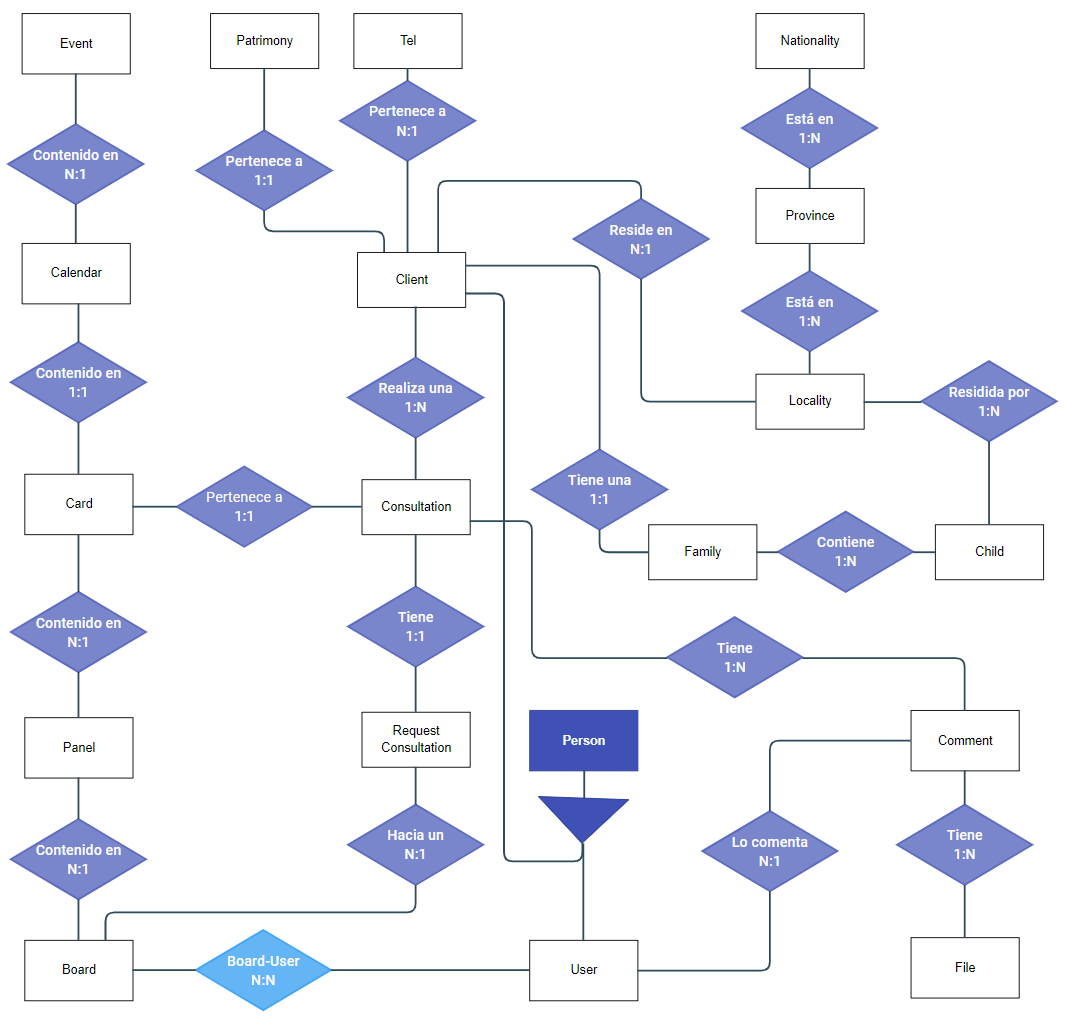
\includegraphics[width=1\linewidth]{fig/der.png}
    \caption{Diagrama Entidad Relación}
    \label{fig:der}
\end{figure}

\newpage

La implementación del modelo se lleva a cabo en Django. Sin embargo, para simplificar la explicación, se han omitido otras entidades relacionadas al usuario propias de Django, como tokens, grupos, etc. A continuación, se presenta el resultado visualizado mediante DBeaver, utilizado como gestor de la base de datos.

\begin{figure}[H]
    \centering
    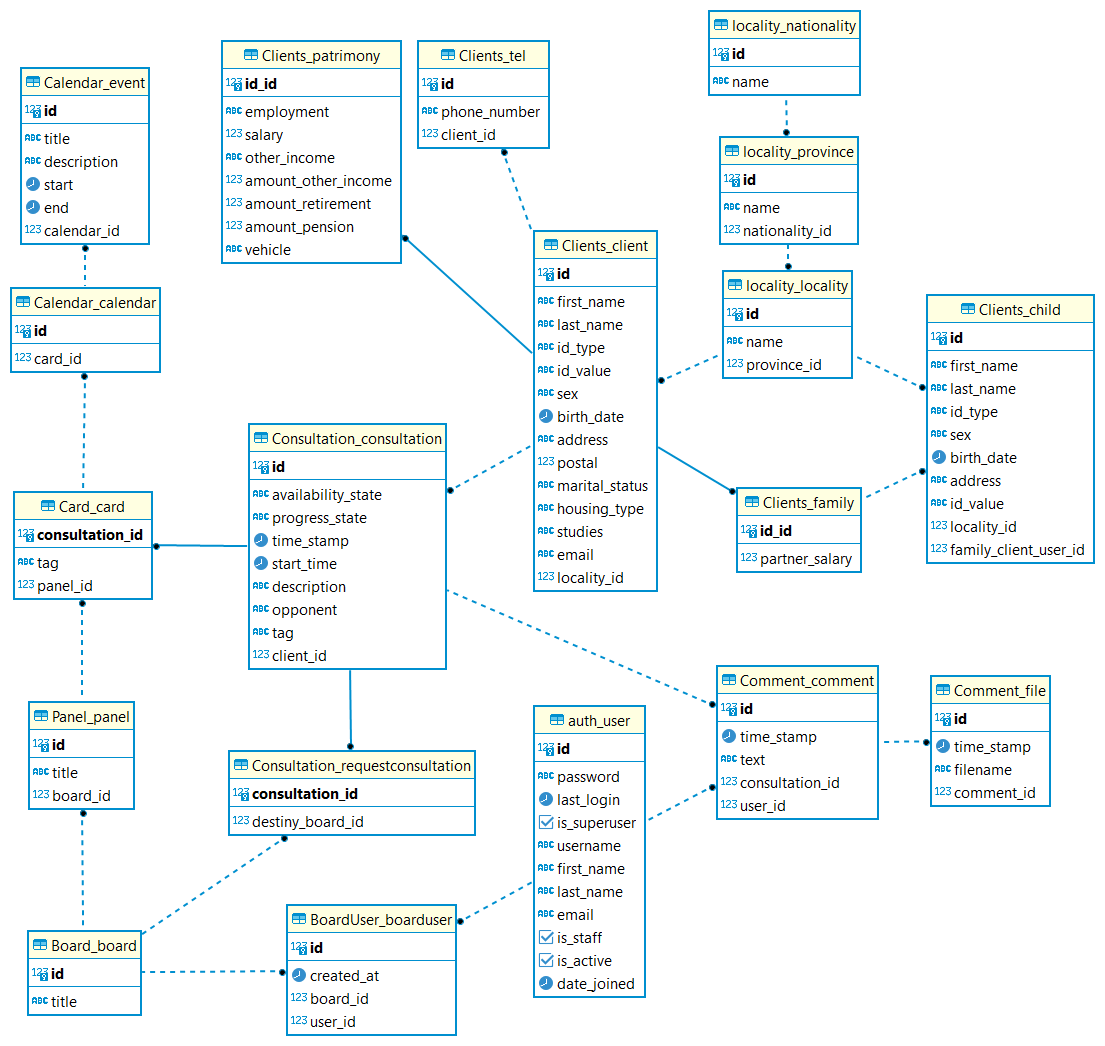
\includegraphics[width=1\linewidth]{fig/dbeaver.png}
    \caption{Implementación del Modelo Entidad Relación}
    \label{fig:dbeaver}
\end{figure}




\section{Requerimientos de Interfaces Externas}


En esta sección, se presenta los requerimientos de de Interfaces, que sirve como un elemento para la visualización y estructuración de la interfaz de usuario. A continuación, se exhiben los mockup representativos del diseño propuesto para la interfaz gráfica de usuario (GUI).

\subsection{Consultoría}

La Figura \ref{fig:gui-consultancy} exhibe un mockup que encapsula la apariencia y disposición previstas de la interfaz de usuario, específicamente en el contexto de la funcionalidad de consultoría.

Dada la necesidad de lograr una experiencia intuitiva, se estableció como requisito la implementación de tableros para la asignación de casos, tomando como referencia la utilización previa de Trello en el organismo.

\begin{figure}[h]
\centering
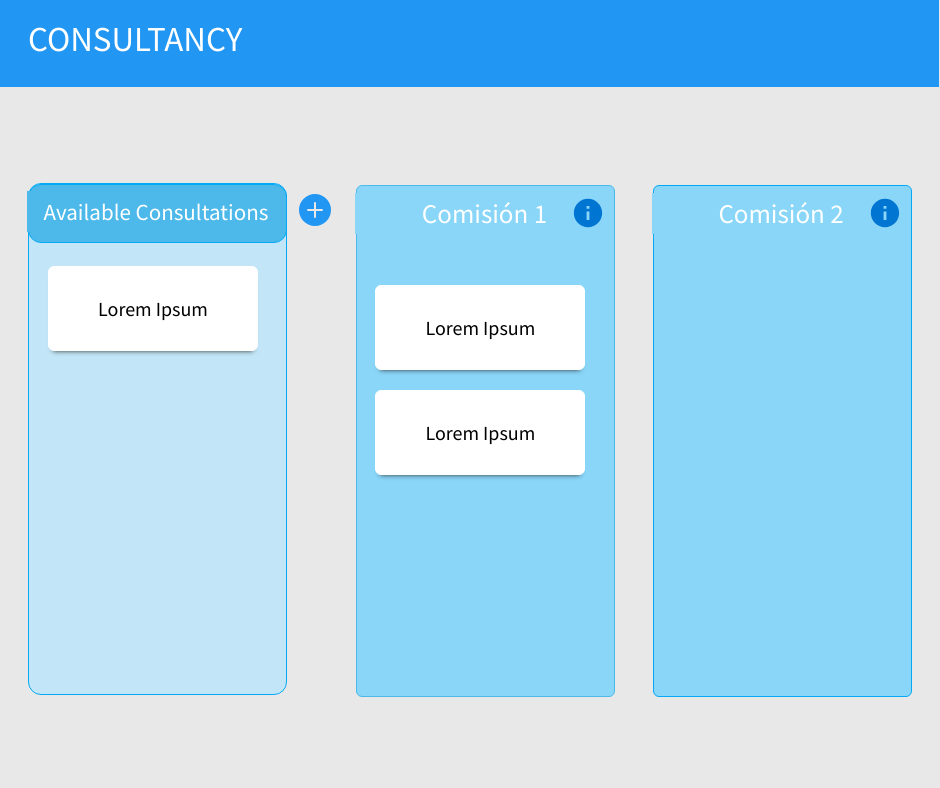
\includegraphics[width=1\linewidth]{fig/GUI-consultancy.png}
\caption{Mockup de la Interfaz Gráfica de Usuario (GUI) para la Página Consultoría}
\label{fig:gui-consultancy}
\end{figure}


A la izquierda, se ubica el tablero de casos sin asignar, mientras que a la derecha se presentan los tableros destinados para enviar las solicitudes de asignación del caso a las diversas comisiones. Cada tarjeta (card) en estos tableros representa una consulta específica.

Adicionalmente, se incorporan dos elementos clave para la interacción:
\begin{itemize}
    \item El botón ``+''  facilita la creación de nuevas consultas.
    \item El botón de información proporciona detalles específicos sobre la comisión correspondiente.
\end{itemize}



\subsection{Tablero de Trabajo para Cada Comisión}

El diseño del tablero de trabajo adopta una lógica similar a la implementada en la funcionalidad de consultoría, manteniendo paneles organizativos que permiten la manipulación intuitiva de tarjetas mediante el sistema de arrastre y soltar.


\begin{figure}[H]
\centering
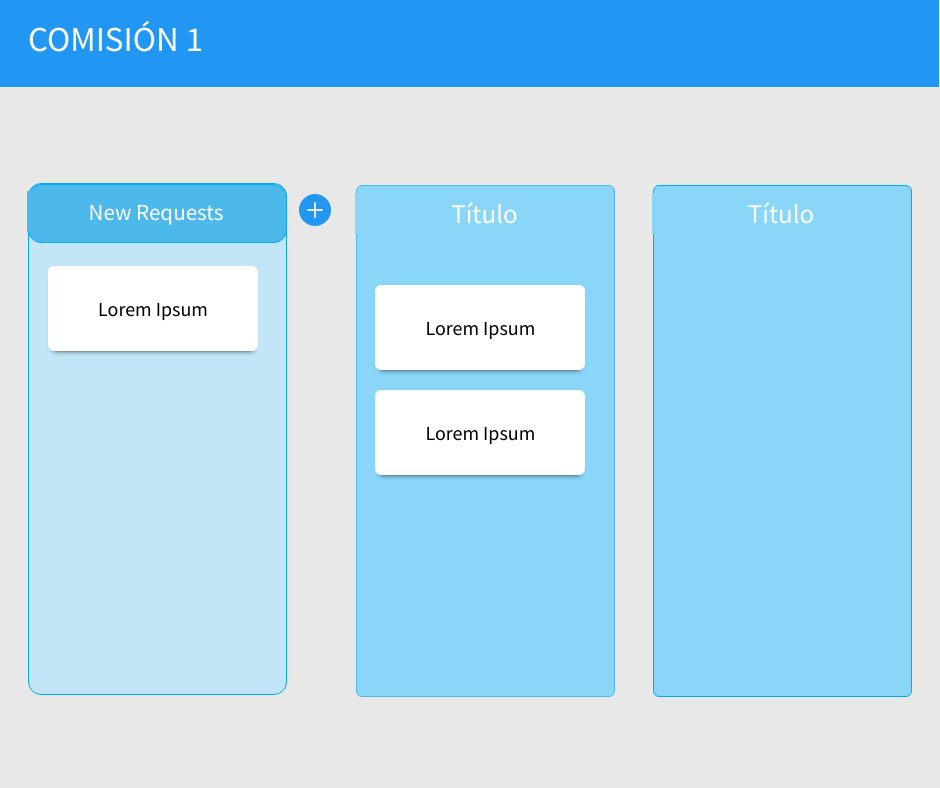
\includegraphics[width=1\linewidth]{fig/board.png}
\caption{Mockup de la Interfaz Gráfica de Usuario (GUI) para el Tablero de Comisión}
\label{fig:board}
\end{figure}


En el lado izquierdo de la imagen, se sitúa el panel de entrada, destinado a recibir las solicitudes entrantes. A la derecha, se encuentran paneles específicos de la comisión, ajustados según las necesidades particulares. La funcionalidad del botón "+" simplifica la creación de paneles adicionales. Por ejemplo, se podrían generar tableros para representar el estado de la consulta o agruparlos según profesor.

Finalmente, las tarjetas blancas dentro de los paneles representan cada consulta con una etiqueta referente.


\subsection{Inicio de Sesión}
Para garantizar la seguridad y autenticación de los usuarios, se ha implementado se tiene como requisito una interfaz de inicio de sesión al sistema. La Figura \ref{fig:enter-label} presenta el diseño visual asociado con la página de inicio de sesión.

\begin{figure}[H]
    \centering
    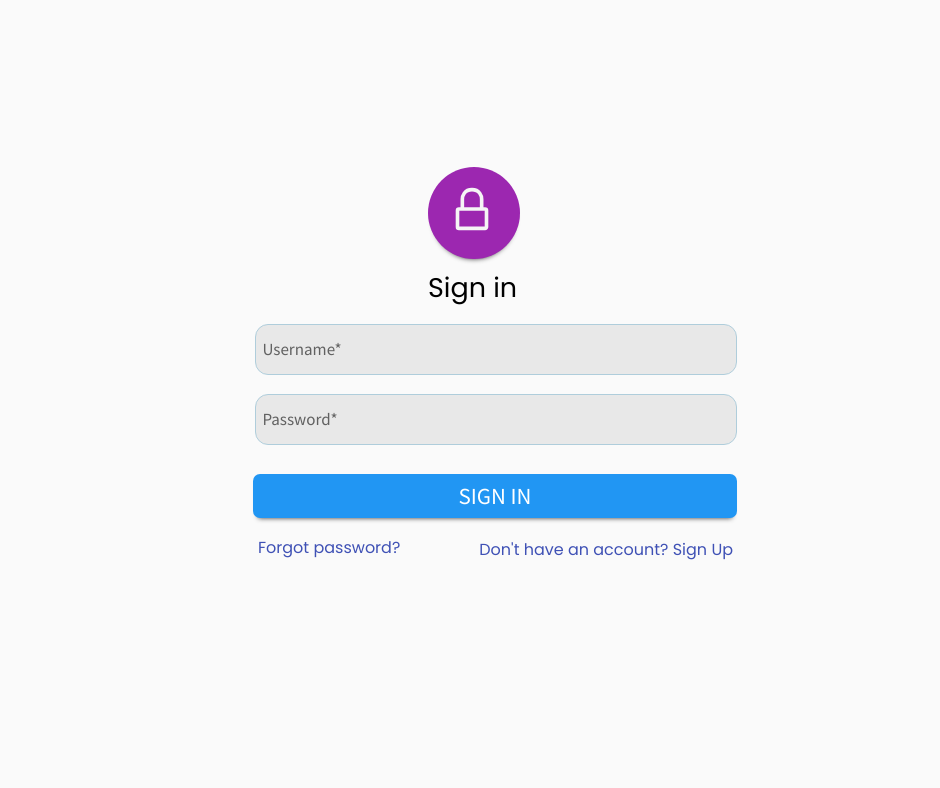
\includegraphics[width=1\linewidth]{fig/signin.png}
    \caption{Mockup de la Interfaz de Inicio de Sesión}
    \label{fig:signin}
\end{figure}

Como se evidencia en esta interfáz, el requisito de inicio de sesión solicita la introducción de un usuario y contraseña para acceder al sistema. Además, se ha incorporado la opción de recuperar la contraseña en caso de olvido, así como la capacidad de crear una nueva sesión para los usuarios que aún no cuentan con una cuenta registrada.


\subsection{Información de la Consulta}

Un requisito fundamental del sistema es la capacidad de visualizar la información detallada de cada consulta. Esta sección abarca diversos aspectos esenciales, incluyendo datos específicos de la consulta, una sección dedicada a comentarios, y una interfaz de calendario para gestionar fechas clave.

La Figura \ref{fig:info-consult-gui} presenta un mockup que ilustra la propuesta visual para la interfaz de información de consulta.

\begin{figure}[H]
\centering
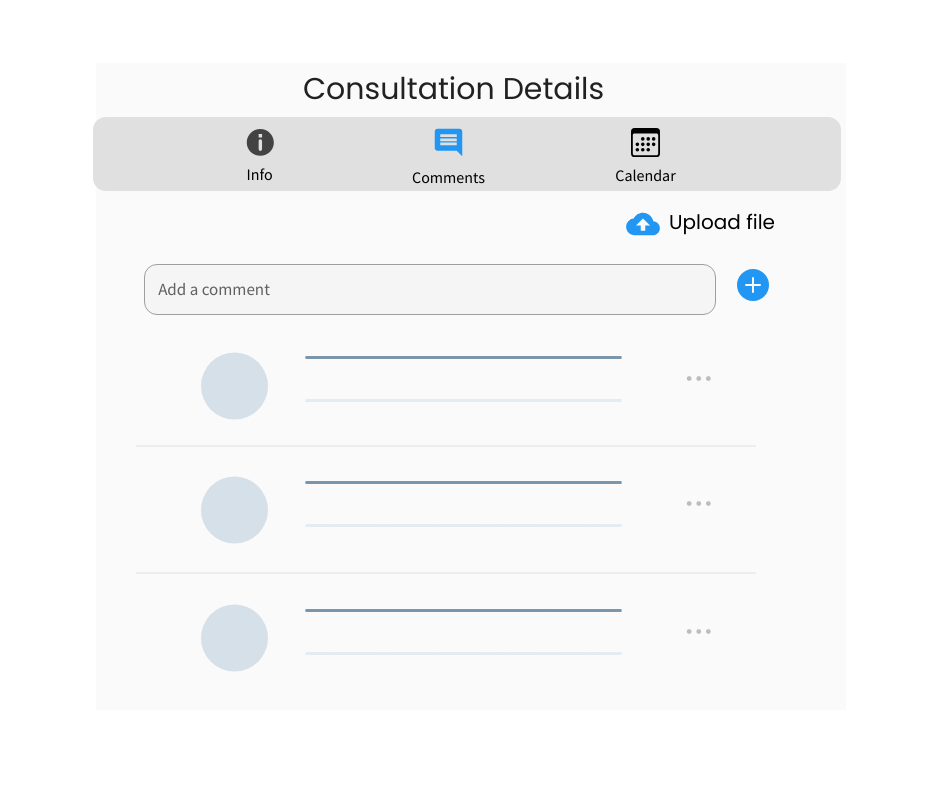
\includegraphics[width=1\linewidth]{fig/comment-gui.png}
\caption{Mockup de la Interfaz de Información de Consulta}
\label{fig:info-consult-gui}
\end{figure}

Esta interfaz permite interactuar a través de la sección de comentarios, permitiendo a los usuarios intercambiar información relevante, registrar datos y adjuntar archivos. Por otro lado, el calendario facilita la organización y seguimiento de eventos asociados a la consulta.

\subsection{Tablas de Control}

Se han requerido tablas para la visualización integral de todos los registros de consultas y clientes. En este contexto, se presenta un ejemplo con la tabla específica de consultas en la Figura \ref{fig:table-consult-gui}.

\begin{figure}[H]
\centering
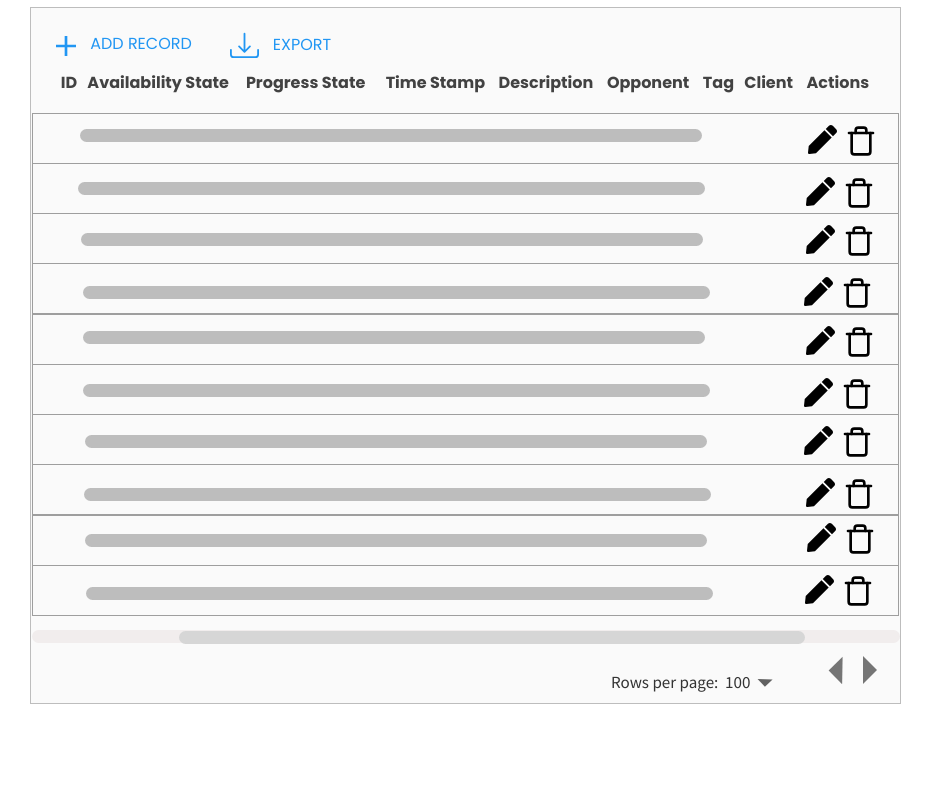
\includegraphics[width=1\linewidth]{fig/table-comment-gui.png}
\caption{Mockup de la Interfaz para las Tablas de Consultas}
\label{fig:table-consult-gui}
\end{figure}



\section{Requerimientos Funcionales}
Según Somerville \cite{Somerville}, Los requerimientos funcionaless son ``Son enunciados acerca de servicios que el sistema
debe proveer, de cómo debería reaccionar el sistema a entradas particulares y de cómo debería comportarse el sistema en situaciones específicas. En algunos casos, los requerimientos funcionales también explican lo que no debe hacer el sistema''

En el marco de este proyecto, los requerimientos funcionales se agrupan según sus funcionalidades específicas:

\begin{table}[H]
\centering
\begin{tabular}{|l|l|}
\hline
\textbf{Referencia} & \textbf{Función} \\
\hline
\textbf{RF.1} & Sistema de solicitudes de asignación de casos \\
\hline
\textbf{RF.2} & Sistema de gestión de casos por comisión \\
\hline
\textbf{RF.3} & Sistema de registro de clientes y consultas \\
\hline
\textbf{RF.4} & Sistema de alertas y notificaciones \\
\hline
\textbf{RF.5} & Registro y Autenticación de Usuarios \\
\hline
\end{tabular}
\caption{Requerimientos Funcionales}
\label{tab:rf}
\end{table}



\subsection{Sistema de Solicitudes de Asignación de Casos}

\begin{table}[H]
    \centering
    \begin{tabular}{|c|p{10cm}|}
        \hline
        \textbf{Referencia} & \textbf{Función} \\
        \hline
        RF.1.1 & Un Tomador de Caso podrá revisar la información de una consulta. \\
        \hline
        RF.1.2 & Un Tomador de Caso podrá revisar la cantidad de casos con sus estados de actividad de una comisión. \\
        \hline
        RF.1.3 & Un Tomador de Caso podrá revisar el historial reciente de solicitudes de una comisión. \\
        \hline
        RF.1.4 & Un Tomador de Caso podrá enviar una solicitud de asignación de un caso a una comisión. \\
        \hline
        RF.1.5 & Un Tomador de Caso podrá deshacer una solicitud de asignación. \\
        \hline
        RF.1.6 & Un Tomador de Caso podrá revisar la totalidad de casos. \\
        \hline
        RF.1.7 & Un Tomador de Caso podrá revisar la totalidad de clientes. \\
        \hline
    \end{tabular}
    \caption{Requerimientos Funcionales para Tomadores de Caso}
    \label{tab:rf-tomadores-caso}
\end{table}



\subsection{Sistema de Gestión de Casos por Comisión}
\begin{table}[H]
    \centering
    \begin{tabular}{|c|p{10cm}|}
        \hline
        \textbf{Requerimiento} & \textbf{Función} \\
        \hline
        RF.2.1 & Un usuario de una comisión tendrá la capacidad de aceptar o rechazar una solicitud de asignación de un nuevo caso a su comisión. \\
        \hline
        RF.2.2 & Un usuario de una comisión podrá visualizar los casos asignados a la comisión, incluyendo su estado y detalles relevantes. \\
        \hline
        RF.2.3 & Un usuario de una comisión podrá realizar modificaciones en los casos asignados a la comisión, actualizando la información según sea necesario. \\
        \hline
        RF.2.4 & Un usuario de una comisión podrá comentar en los casos asignados a la comisión, proporcionando información adicional o aclaraciones con la posibilidad de adjuntar archivos. \\
        \hline
        RF.2.5 & Un usuario de una comisión tendrá la opción de agregar y quitar eventos en los casos asignados a la comisión, permitiendo un seguimiento detallado de las actividades relacionadas con cada caso. \\
        \hline
    \end{tabular}
    \caption{Requerimientos Funcionales del Sistema de Gestión de Casos por Comisión}
    \label{tab:rf-gestion-casos-comision}
\end{table}

\subsection{Sistema de Registro de Clientes y Consultas}

\begin{table}[H]
    \centering
    \begin{tabular}{|l|p{10cm}|}
        \hline
        \textbf{Requerimiento} & \textbf{Descripción} \\
        \hline
        RF.3.1 & Un Tomador de Caso o Super Usuario podrá almacenar los datos de un cliente en el sistema. \\
        \hline
        RF.3.2 & Un Tomador de Caso o Super Usuario podrá registrar los detalles de una consulta de un cliente en el sistema. \\
        \hline
        RF.3.3 & El sistema permitirá cargar clientes mediante la integración con Google Forms, agilizando el ingreso de datos al sistema. \\
        \hline
        RF.3.4 & El sistema permitirá cargar consultas mediante la integración con Google Forms, facilitando el registro eficiente de información relacionada con las consultas de los clientes. \\
        \hline
    \end{tabular}
    \caption{Requerimientos del Sistema de Registro de Clientes y Consultas}
    \label{tab:registro-clientes-consultas}
\end{table}


\subsection{Sistema de Notificaciones y Alertas}

\begin{table}[H]
    \centering
    \begin{tabular}{|l|p{10cm}|}
        \hline
        \textbf{Requerimiento} & \textbf{Descripción} \\
        \hline
        RF.4.1 & El sistema podrá enviar correos electrónicos para notificar a los Tomadores de Caso cuando una solicitud es aceptada o rechazada. \\
        \hline
        RF.4.2 & El sistema podrá enviar correos electrónicos a los usuarios de una comisión al llegar una nueva solicitud de asignación de caso. \\
        \hline
        RF.4.3 & El sistema enviará alertas en tiempo real a los Tomadores de Caso cuando una solicitud es aceptada o rechazada. \\
        \hline
        RF.4.4 & El sistema enviará alertas a los usuarios de una comisión al llegar una solicitud de asignación de caso. \\
        \hline
        RF.4.5 & El sistema enviará alertas cuando ingresa un nuevo cliente o consulta a través de Google Forms, manteniendo a los usuarios informados sobre las actualizaciones en el sistema. \\
        \hline
    \end{tabular}
    \caption{Requerimientos del Sistema de Notificaciones y Alertas.}
    \label{tab:notificaciones-alertas}
\end{table}

\subsection{Registro y Autenticación de Usuarios}

\begin{table}[H]
    \centering
    \begin{tabular}{|l|p{10cm}|}
        \hline
        \textbf{Requerimiento} & \textbf{Descripción} \\
        \hline
        RF.5.1 & Un usuario podrá acceder a la plataforma mediante un nombre de usuario y contraseña. \\
        \hline
        RF.5.2 & Un usuario podrá registrarse en la plataforma a través de un proceso de autenticación vía correo electrónico. El acceso a la plataforma estará condicionado a la aceptación por parte de un usuario administrador. \\
        \hline
        RF.5.3 & Un usuario tendrá la capacidad de cambiar su contraseña en caso de olvidarla. \\
        \hline
        RF.5.4 & La plataforma permitirá a los usuarios visualizar únicamente las páginas para las cuales tengan permisos. \\
        \hline
    \end{tabular}
    \caption{Requerimientos de Registro y Autenticación de Usuarios.}
    \label{tab:registro-autenticacion}
\end{table}

\section{Requerimientos No Funcionales}
Según Somerville \cite{Somerville}, los requerimientos no funcionales son ``Son limitaciones sobre servicios o funciones que
ofrece el sistema. Incluyen restricciones tanto de temporización y del proceso de
desarrollo, como impuestas por los estándares. Los requerimientos no funcionales
se suelen aplicar al sistema como un todo, más que a características o a servicios
individuales del sistema.''

\begin{table}[H]
\centering
\begin{tabular}{|l|l|}
\hline
\textbf{Referencia} & \textbf{Función} \\
\hline
\textbf{RNF.1} & Requerimientos del producto \\
\hline
\textbf{RNF.2} & Requerimientos de la organización \\
\hline
\textbf{RNF.3} & Requerimientos externos \\
\hline
\end{tabular}
\caption{Requerimientos No Funcionales}
\label{tab:rnf}
\end{table}

\subsection{Requerimientos del producto}

\begin{table}[H]
    \centering
    \begin{tabular}{|l|p{10cm}|}
        \hline
        \textbf{Requerimiento} & \textbf{Descripción} \\
        \hline
        RNF.1.1 & El sistema se podrá acceder a través de la web desde una computadora con acceso a internet. \\
        \hline
        RNF.1.2 & La interfaz de usuario deberá ser intuitiva y fácil de usar, siguiendo los principios de diseño de experiencia de usuario (UX). \\
        \hline
        RNF.1.3 & El sistema deberá ser capaz de manejar simultáneamente por 5 a 10 usuarios sin degradación del rendimiento. \\
        \hline
        RNF.1.4 & El acceso a ciertas funcionalidades estará restringido a usuarios autorizados mediante roles y permisos. \\
        \hline
    \end{tabular}
    \caption{Requerimientos del Producto.}
    \label{tab:rnf-producto}
\end{table}

\subsection{Requerimientos de la organización}

\begin{table}[H]
    \centering
    \begin{tabular}{|l|p{10cm}|}
        \hline
        \textbf{Requerimiento} & \textbf{Descripción} \\
        \hline
        RNF.2.1 & La PC del usuario deberá tener un mínimo de 4GB de RAM y tarjeta de red para la conexión a internet. \\
        \hline
        RNF.2.2 & La plataforma será compatible con versiones estables de Chrome \(>=\) 120.0.6099.* y accesible a través de pantallas medianas a grandes. \\
        \hline
        RNF.2.3 & El código fuente deberá seguir buenas prácticas de desarrollo y ser fácilmente mantenible. \\
        \hline
    \end{tabular}
    \caption{Requerimientos de la Organización.}
    \label{tab:rnf-organizacion}
\end{table}

\subsection{Requerimientos externos}

\begin{table}[H]
    \centering
    \begin{tabular}{|l|p{10cm}|}
        \hline
        \textbf{Requerimiento} & \textbf{Descripción} \\
        \hline
        RNF.3.1 & Un usuario deberá aceptar los términos y condiciones para el registro a la plataforma. \\
        \hline
        RNF.3.2 & El sistema debe aplicar una política de complejidad de contraseñas que incluya la longitud mínima, uso de mayúsculas, minúsculas, números y caracteres especiales. \\
        \hline
        RNF.3.3 & Se debe implementar una protección efectiva contra ataques de fuerza bruta en las interfaces administrativas, incluyendo mecanismos de bloqueo temporal de cuentas. \\
        \hline
        RNF.3.4 & La integración con Google Forms y la API debe utilizar tokens de seguridad para autenticar y autorizar las solicitudes, manteniendo un flujo seguro de información. \\
        \hline
        RNF.3.5 & La plataforma deberá implementar medidas de seguridad contra ataques CSRF Token. \\
        \hline
        RNF.3.6 & La comunicación entre el servidor y los usuarios debe estar cifrada mediante un certificado SSL proporcionado por Let's Encrypt y configurado en el servidor Nginx. \\
        \hline
    \end{tabular}
    \caption{Requerimientos Externos.}
    \label{tab:rnf-externos}
\end{table}


\section{Definición de Roles y Responsabilidades}

\begin{table}[H]
    \centering
    \begin{tabular}{|p{3cm}|p{12cm}|}
        \hline
        \textbf{Tomador de Caso} & Este usuario tiene acceso al tablero de la consultoría y al panel de control. Su responsabilidad principal es agregar clientes y consultas de forma manual, además de asignar las consultas a una comisión específica. Los Tomadores de Caso pueden visualizar el estado de cada comisión, revisando la cantidad de casos activos y las últimas solicitudes enviadas.\\
        \hline
        \textbf{Integrante de Comisión (Profesor)} & Este rol se asigna a los integrantes de una comisión con acceso al tablero. Sus responsabilidades incluyen aceptar o rechazar solicitudes de asignación de casos o consultas. Además, se encargan de gestionar el seguimiento y progreso de cada caso asignado a su comisión.\\
        \hline
        \textbf{Jefe de Patrocinio (Administrador)} & También conocido como administrador, este usuario tiene privilegios que le otorgan acceso total a la plataforma. Sus responsabilidades principales incluyen la gestión de usuarios, permisos y roles, asegurando el correcto funcionamiento y la seguridad de la plataforma.\\
        \hline
        \textbf{Cliente (por Google Forms)} & Consultante que busca patrocinio gratuito. Este actor no tiene acceso directo a la plataforma y no ingresa a ella. Su interacción se limita a completar formularios de registro de cliente y consulta, los cuales se cargan automáticamente en la plataforma desde \textbf{Google Forms}.\\
        \hline

    \end{tabular}
    \caption{Roles y Responsabilidades de los Actores en la Plataforma}
    \label{tab:roles-responsabilidades}
\end{table}


\section{Diagrama de Caso de Uso del Sistema}
A continuación, se presentan los diagramas de caso de uso \ref{fig:caso-de-uso} para identificar a los actores implicados en una interacción. Si bien en este caso no se relacionan los casos de uso a alto nivel con diferentes actores, no significa que no exista una relación. Por otro lado, debe entenderse que Google Forms también cumple un rol e interactúa con el sistema principal Case Management System.

\begin{figure}[H]
\centering
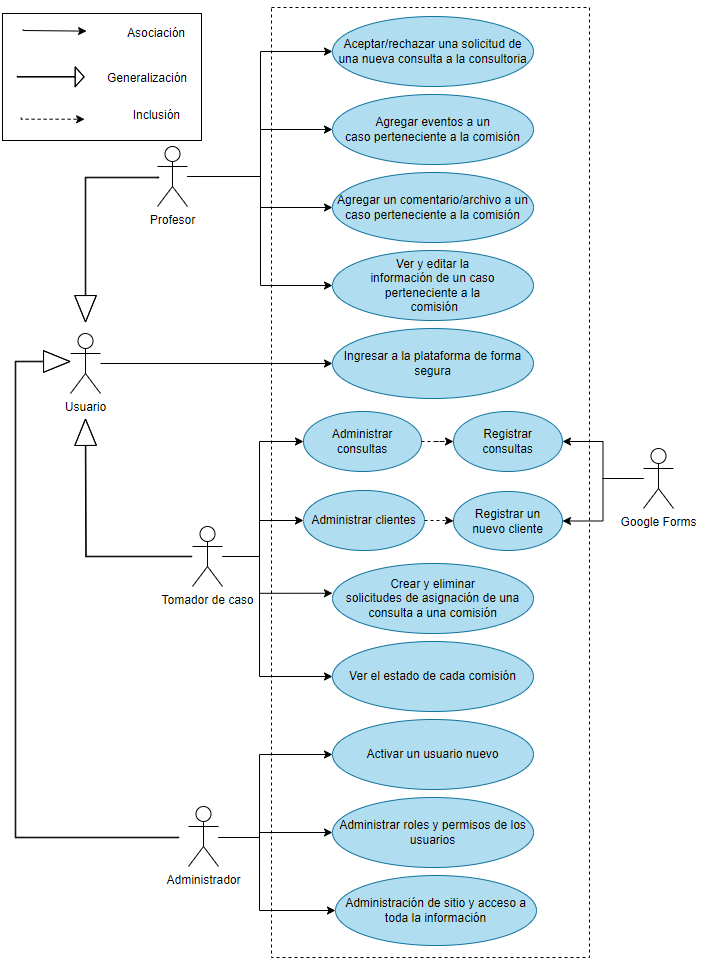
\includegraphics[width=1\linewidth]{fig/caso-de-uso.png}
\caption{Diagrama Caso de Uso}
\label{fig:caso-de-uso}
\end{figure}

\begin{itemize}
\item \textbf{CU.1}: Aceptar/rechazar una solicitud de una nueva consulta a la consultoría.
\item \textbf{CU.2}: Agregar eventos a un caso perteneciente a la comisión.
\item \textbf{CU.3}: Agregar un comentario/archivo a un caso perteneciente a la comisión.
\item \textbf{CU.4}: Ingresar a la plataforma de forma segura.
\item \textbf{CU.5}: Administrar consultas.
\item \textbf{CU.6}: Administrar clientes.
\item \textbf{CU.7}: Crear y eliminar solicitudes de asignación de una consulta a una comisión.
\item \textbf{CU.8}: Ver el estado de cada comisión.
\item \textbf{CU.9}: Activar a un usuario nuevo.
\item \textbf{CU.10}: Administrar roles y permisos de los usuarios.
\item \textbf{CU.11}: Administración de sitio y acceso a toda la información.
\end{itemize}


\section{Diagrama de Secuencia Nominal Simplificado}
A continuación, se incluye un diagrama de secuencia \ref{fig:secuencia-nominal} simplificado de alto nivel que representa una secuencia nominal para agregar comprensión a la funcionalidad de cada actor y su interacción con otros actores.

\begin{figure}[H]
\centering
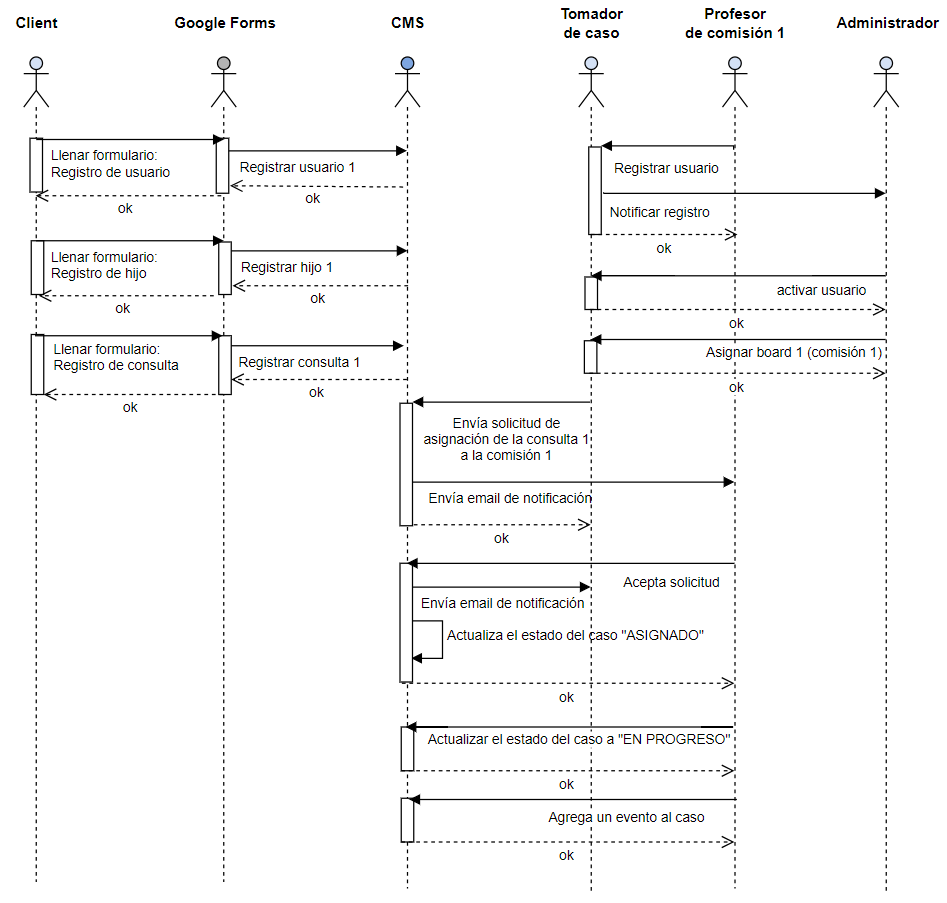
\includegraphics[width=1\linewidth]{fig/secuencia-basica.png}
\caption{Diagrama de Secuencia Simplificado}
\label{fig:secuencia-nominal}
\end{figure}

En este diagrama, participan varios actores, incluyendo un cliente con un solo hijo, el sistema externo Google Forms, el sistema Case Management System, el usuario tomador de caso, el profesor de la comisión número uno y el jefe de patrocinio o administrador.

Además, se detallan dos eventos en paralelo: el registro de un usuario en la plataforma y el registro de un cliente con una nueva consulta.

\section{Matriz de Trazabilidad}
La siguiente matriz de trazabilidad relaciona cada uno de los requerimientos con los casos de uso.

\begin{table}[H]
    \centering
    \small
    \begin{tabular}{|c|@{}c|@{}c|@{}c|@{}c|@{}c|@{}c|@{}c|@{}c|@{}c|@{}c|@{}c|}
    \hline
               & \textbf{CU1} & \textbf{CU2} & \textbf{CU3} & \textbf{CU4} & \textbf{CU5} & \textbf{CU6} & \textbf{CU7} & \textbf{CU8} & \textbf{CU9} & \textbf{CU10} & \textbf{CU11}\\
    \hline
    \hline
        \textbf{RF.1.1} &  &  & & &  & $\bullet$&  &  &  & & \\
        \hline
        \textbf{RF.1.2} &  &  & & &  &  &  &  & $\bullet$ & & \\
        \hline
        \textbf{RF.1.3} &  &  & &  &  &  &  &  & $\bullet$ & & \\
        \hline
        \textbf{RF.1.4} &  &  & &  &  &  &  & $\bullet$ &  & & \\
        \hline
        \textbf{RF.1.5} &  &  & &  &  &  &  & $\bullet$ &  & & \\
        \hline
        \textbf{RF.1.6} &  &  & &  &  & $\bullet$ &  &  &  & & \\
        \hline
        \textbf{RF.1.7} &  &  & &  &  &  &  $\bullet$ &  &  & & \\
        \hline
        \textbf{RF.2.1} & $\bullet$ &  &  & &  &  &  &  &  & & \\
        \hline
        \textbf{RF.2.2} &  &  &  & & $\bullet$ &  &  &  &  & & \\
        \hline
        \textbf{RF.2.3} &  &  & & & $\bullet$ &  &  &  &  & & \\
        \hline
        \textbf{RF.2.4} &  &  & $\bullet$ & & &  &  &  &  & & \\
        \hline
        \textbf{RF.2.5} &  & $\bullet$ &  & & &  &  &  &  & & \\
        \hline
        \textbf{RF.3.1} &  &  &  & &  &  & $\bullet$ &  &  & & $\bullet$ \\
        \hline
        \textbf{RF.3.2} &  &  &  & & & $\bullet$ &  &  &  & & $\bullet$ \\
        \hline
        \textbf{RF.3.3} &  &  &  & & &  & $\bullet$ &  &  & & \\
        \hline
        \textbf{RF.3.4} &  &  &  & & & $\bullet$ &  &  &  & & \\
        \hline
        \textbf{RF.4.1} & $\bullet$ & & &  &  &  &  &  &  & & \\
        \hline
        \textbf{RF.4.2} &  &  & & &  &  &  & $\bullet$ &  & & \\
        \hline
        \textbf{RF.4.3} & $\bullet$ &  & &  &  &  &  &  &  & & \\
        \hline
        \textbf{RF.4.4} &  &  &  & &  &  &  & $\bullet$ &  & & \\
        \hline
        \textbf{RF.4.5} &  &  &  & & &  & $\bullet$ &  &  & & \\
        \hline
        \textbf{RF.5.1} &  &  &  & $\bullet$ & &  &  &  &  & & \\
        \hline
        \textbf{RF.5.2} &  &  &  & $\bullet$ & &  &  &  & & & \\
        \hline
        \textbf{RF.5.3} &  &  &  & $\bullet$ &  &  &  &  &  & & \\
        \hline
        \textbf{RF.5.4} &  &  &  &&  &  &  &  &  & $\bullet$ & \\
    \hline
        \textbf{RNF.1.1} &  &  & & &  &  &  &  &  & & \\
        \hline
        \textbf{RNF.1.2} &  &  & & &  &  &  &  &  & & \\
        \hline
        \textbf{RNF.1.3} &  &  & & &  &  &  &  &  & & \\
        \hline
        \textbf{RNF.1.4} &  &  & & &  &  &  &  &  & $\bullet$ & \\
        \hline
        \textbf{RNF.2.1} &  &  & & &  &  &  &  &  & & \\
        \hline
        \textbf{RNF.2.2} &  &  & & &  &  &  &  &  & & \\
        \hline
        \textbf{RNF.2.3} &  &  & & &  &  &  &  &  & & \\
        \hline
        \textbf{RNF.3.1} &  &  & & &  &  &  &  &  & & \\
        \hline
        \textbf{RNF.3.2} &  &  &&  &  &  &  &  &  & & \\
        \hline
        \textbf{RNF.3.3} &  &  & & &  &  &  &  &  & & \\
        \hline
        \textbf{RNF.3.4} &  &  & & &  &  &  &  &  & & \\
        \hline
        \textbf{RNF.3.5} &  &  & & &  &  &  &  &  & & \\
        \hline
        \textbf{RNF.3.6} &  &  &  & &  &  &  &  &  & & \\
    \hline
    \end{tabular}
    \caption{Matriz de Trazabilidad}
    \label{tab:matriz-trazabilidad}
\end{table}

